\documentclass{article}

% if you need to pass options to natbib, use, e.g.:
% \PassOptionsToPackage{numbers, compress}{natbib}
% before loading nips_2016
%
% to avoid loading the natbib package, add option nonatbib:
% \usepackage[nonatbib]{nips_2016}

\PassOptionsToPackage{numbers,sort&compress}{natbib}
\usepackage[final]{nips_2016} % produce camera-ready copy

\usepackage[utf8]{inputenc} % allow utf-8 input
\usepackage[T1]{fontenc}    % use 8-bit T1 fonts
\usepackage{hyperref}       % hyperlinks
\usepackage{url}            % simple URL typesetting
\usepackage{booktabs}       % professional-quality tables
\usepackage{amsfonts}       % blackboard math symbols
\usepackage{nicefrac}       % compact symbols for 1/2, etc.
\usepackage{microtype}      % microtypography

\usepackage{amsmath}        %added by s2713107 for equations and array names
\usepackage{graphicx}       %added by s2713107 for graphs
\usepackage{float}          %added by s2713107 for graph placement
\usepackage{booktabs}       %added by s2713107 for tables

\title{Developing a machine learning tool to predict ecologically suitable areas within the United States to translocate at-risk species}

% The \author macro works with any number of authors. There are two
% commands used to separate the names and addresses of multiple
% authors: \And and \AND.
%
% Using \And between authors leaves it to LaTeX to determine where to
% break the lines. Using \AND forces a line break at that point. So,
% if LaTeX puts 3 of 4 authors names on the first line, and the last
% on the second line, try using \AND instead of \And before the third
% author name.

\author{
  s2013679\\
  %% examples of more authors
  \And
  s2713107\\
 \And
  s2691680\\
 \And
  s2762009
}

\begin{document}

\maketitle

\begin{abstract}
This report focuses on the task of finding an appropriate location to which a given species can be translocated as part of conservation efforts. Ecological features were added to species observation data, and used to classify and cluster coordinates in the United States of America (USA) which were environmentally suitable targets for translocation for a target species. This report aims to handle the nature of species observation data lacking absences, containing outliers, and being imbalanced. Best performance was achieved by training an Adaptive Boosted decision tree model with observation data containing pseudo-absences, combined with clustering species co-occurrence to predict coordinates in the known range of a target species, but outside of the observed range.\end{abstract}

\section{Introduction}
Extreme weather conditions and natural hazards are predicted to become more frequent as the climate warms. \cite{goncalves_global_2024}. A proposed conservation strategy is translocation, moving a species considered at risk from a source population to a new habitat. Translocation has been shown to be successful when performed for conservation purposes, and several success stories have been reported including the restoration of \textit{(Egretta thula)} populations in Louisiana and Florida \cite{spatz_tracking_2023}. Recently, the U.S. Fish and Wildlife Service (FWS) revised a section of the Endangered Species Act, allowing reintroduction of experimental populations outside their ‘historic range’ \cite{fws}. Translocation is a risky strategy due to the ecological and socioeconomic impact that the source species may have on the target area, so risk assessment frameworks include an assessment of the suitability of the target location to the source population to reduce the risk involved in translocation \cite{hoegh-guldberg_assisted_2008}.

Species distribution models (SDMs) provide an evidence-based approach to predict the ecological suitability for a species to a given habitat\cite{guisan_predicting_2013}. We propose a tool that is trained on publicly available species occurrence data uploaded to iNaturalist.org, habitat type and elevation data to learn to identify locations that have suitable characteristics for relocation of an at-risk population. This model was developed specifically for species observed in Florida in the southeastern U.S. as a region with habitats of ecological interest that are at risk from extreme weather.

\section{Data preparation}

All coding tasks in this project were performed on Python 3. Data and code relevant in this report can be found in the Appendix (Section \ref{appendix}).

\subsection{Description of the data}

Provided data was given in the form of numpy arrays \cite{numpy}. Training data was formatted as rows of coordinates (latitude, longitude) with matching species IDs from the iNaturalist observation database \cite{inaturalist}. The data is restricted to species presences, lacking a measure of absences. It also suffers from observation bias and sampling errors due to the data being collected from the devices of a multitude of users that are likely restricted to easily accessible locations. 
The test data from the IUCN red list of threatened species \cite{iucndata} is a series of regularly inter-spaced coordinates that map out the surface of the Earth which were labeled with species IDs to signify their presence.

The data was adapted and complemented to obtain three similarly structured datasets used in this report. The training dataset features coordinate-species pairs for all species observed in Florida throughout the US, with a binary "presence" column to be used as target in machine learning (1 = presence, 0 = absence). Complementary columns have been added to be used as features: Köppen-Geiger (KG) climate classification (e.g. Cfa and Cwa represent humid subtropical climates \cite{KG}), and elevation zones (ordinal categorisation of altitude ranges). A prediction dataset designed to generate predictions for relevant coordinates was generated from the IUCN data. It maps out U.S. coordinates with the same feature columns as before. The test dataset designed for model evaluation contains the same columns as the training dataset, and describes all species throughout the U.S. in the IUCN data.  

The following subsections offer an overview of the key data manipulations used to produce these datasets.

\subsection{Climate labeling and geographical filtering}
The KG classification data\cite{KG} was appended to the test and training coordinates using a KNeighborsClassifier from Python package scikit-learn \cite{scikit-learn} on the KG-labelled coordinates (features: coordinates; target: label; n\_neighbors = 1) to generate label approximations for training and test coordinates as the nearest neighbouring values.
 We then used the package reverse\_geocoder \cite{rev-geo} to filter for Floridian species (training data only) and USA coordinates, using country and state data matched to the coordinates. These steps would yield early versions of the training and prediction data.

\subsection{Fetching elevation data}
From the relevant coordinates selected above, we fetched matching elevation data by sending GET queries to the open-elevation API \cite{open-elevation} iteratively. The API takes query coordinates and returns the corresponding elevation from the Shuttle Radar Topography Mission (SRTM) data \cite{SRTM}. There are two notable complications with this approach. Firstly, unknown data-points are given a default elevation of 0.0, which risks creating false values; the API may also return empty values, seemingly due to responsiveness issues. Although we did not compensate for the risk of false 0.0 values, we found it possible to eliminate empty values by running the elevation-querying code again on coordinates with missing values.

To simplify the data passed to the supervised model and give more meaning to ranges of altitudes we sorted elevation values into ordinal levels ranging from 0 to 9. These levels  were arbitrarily defined to cover altitudes that range from negative to above 3000m, following a naive approach inspired by Ch.3 of The Biology of Alpine Habitats \cite{elevation-gradients}, describing the difference elevation gradients make in ecosystems, and Ch. 21 \cite{ch21} and 33 \cite{ch33} of \textit{Ecological Subregions of the United States}. See Appendix Figure \ref{fig:elevations} to visualise elevation levels.


\subsection{Defining absences for presence-only data}
When predicting species distribution data, a machine learning tool should be able to discriminate between presence and absence, so both are required for effective learning. To compensate for the common lack of empiric absence data, methods of generating pseudo-absences have been established in the literature \cite{pa-review}. Although these can be randomly generated, preferably in regions defined by environmental filters for relevance, choosing pseudo-absences with the same spatial bias as the original presence samples is better supported. This can be achieved by using the occurrence data of different species in the regions of interest \cite{pa-samebias}. 

We established a method of "box difference" selection to follow this principle by selecting presence data of different species that doesn't overlap with a species of interest's (SOI) distribution. We first defined the entire area A covered by Floridian species in the USA as a two-dimensional box (rectangle) of coordinates using shapely \cite{shapely}. We then identified a smaller box S covering the distribution of a given SOI. Then we assigned all observations that fall within the difference D between these two boxes as pseudo-absences (0) for the SOI (repeat for all species until the dataset is complete). A diagram of the method used is available in the Appendix (Figure \ref{fig:absences}).

To produce the test dataset, we  looped through the prediction coordinates and assigned presences for matching species in the original data. Then, to get absences, we looped through species present in this presence data and assigned absences to coordinates that were not matched to each species, preserving climate and elevation labels.

\section{Learning methods}
\subsection{Exploration of species-location relationships using clustering}\label{clustering_loc}

This model explores sub-populations of target species chosen earlier in Florida. Knowing regional species populations allows to identify which groups might have been in close proximity to natural hazards. This model compares three machine learning algorithms: k-means, k-medoids and hierarchal clustering using silhouette score to determine the most suitable approach for the given species data, then visualises clusters created with the model with the highest silhouette score.

K-means clustering randomly assigns each data point to a cluster and then computes the centroids. This is followed by measurement of the distance between each data point and centroid and then reassignment to the closest centroid. Centroids are recalculated after each iteration until all observations are assigned to the closet centroid. \cite{datacamp_ml} The K-means algorithm is highly efficient which makes it suitable for great data sets. Its main disadvantages include a tendency to favour spherical clusters which may not be appropriate for all sorts of data and sensitivity for outliers. K-Medoids algorithm works similarly to K-Means, but it chooses one of the data points as a medoid instead of finding centroids. This is slower, but less sensitive to outliers as extreme values don’t affect the mean needed to find a centroid. \cite{geeksforgeeks_kmeans} Agglomerative clustering is a type of hierarchal clustering used by this model. At first, it treats all data points as separate clusters, then merges clusters within proximity. This is continued until the target number of clusters is obtained or all observations are merged into one cluster. Unlike in k-means and k-medoids algorithms, there is no need to set the number of clusters before and if the distance threshold is set instead – clusters will stop merging when that distance between clusters is reached. \cite{geeksforgeeks_hierarchical, scikit_agglomerative} Hierarchical clustering is more suitable for smaller data sets as it is very computationally expensive.

Silhouette Score was used to evaluate the performance of algorithms described above on target species in Florida. This is calculated by obtaining the mean distance from each point to other points in the same cluster, and the mean distance between each point and points in the next nearest cluster. The overall silhouette score is the mean of silhouette scores from all points in the cluster, ranging from -1 to 1, where 1 indicates well-defined clusters. Alternative methods of cluster evaluation include an Elbow Plot for k-means clustering and a dendrogram for hierarchical clustering. Criticism of Elbow plots \cite{milligan1985clusters, ketchen1996cluster, schubert2023elbow} include a decrease in the sum of squared errors (SSE) as the number of clusters (k) increases, which often results in model failure on Real-World data sets. Therefore, this model uses the Silhouette Score as a more reliable alternative. Dendrogram might be used to visualise the distances between clusters, but it was not added due to space constraints. This model uses the Silhouette Score to evaluate different numbers of clusters in hierarchal clustering. 
 
\subsection{Classification using Decision Trees}
To predict presence for a target species, a decision tree was trained to classify coordinates into present (1) or absent (0) classes using elevation and one-hot encoded KG classes as features. The initial tree tested species \textit{Tadarida brasiliensis}, which is an imbalanced subset of the data with 16.27\% positive class in the training dataset, and presence is confined to the south and western US. F1-score was calculated as the harmonic means of sensitivity and precision. $F1 = \frac{2*Precision*Recall}{Precision+Recall} = \frac{2*TP}{2*TP+FP+FN}$. This was chosen as the metric to tune classifiers as it ignores true negatives, which are pseudo-absences only. Each split in the tree was decided by minimum Gini index, which was shown in evaluation to be as effective as minimum entropy, but less computationally expensive. Before balancing classes, the model overestimates absence data, which is the majority class. After balancing and pruning to 17 layers from an evaluation of depth from 2 to 30 layers using sklearn's GridSearchCV \cite{scikit-learn}, the F1 score improved from 0.24 to 0.58. The model successfully identifies the broad distribution of \textit{Tadarida brasiliensis}, with decreased accuracy from 0.55 to 0.49, with more false positives present in the prediction. This is preferred as it gives more possible areas for relocation, while eliminating areas that are very unsuitable.

To minimise the error made by a single tree, ensemble trees were trained from Python package scikit-learn \cite{scikit-learn}using the same species, with the tuned Decision Tree Classifier as a base estimator, class weights balanced and random state set to 42. These models train multiple trees which are consolidated into a single output. Random forest models train trees in parallel, while the Adaptive boost (AdaBoost) and gradient boosted models train trees sequentially and are able to learn from previous trees\cite{ensembles}. AdaBoost model assigns sample weights at each iteration to focus on increasingly difficult to classify examples, and gradient boosting uses each new model to minimise the loss function, which here was measured by log loss \cite{rahman}. Accuracy is calculated as $Accuracy = \frac{TP+TN}{TP+TN+FP+FN}$, and is shown here to illustrate the trade-off between the true positive rate and false negative rate.
\begin{table}[ht]
\centering
\begin{tabular}{lcccc}
\toprule
\textbf{Method} & \textbf{Accuracy} & \textbf{F1}  & \textbf{Accuracy after tuning} & \textbf{F1 after tuning}     \\
\midrule
\texttt{Decision Tree Classifier}       & 0.55& 0.24&0.49&0.58 \\ 
\texttt{Random Forest Classifier}     & 0.55 & 0.25 & 0.54 & 0.62 \\ 
\texttt{ADABOOST}  & 0.64& 0.67 & 0.64&0.67 \\ 
\texttt{Gradient Boosting} & 0.54& 0.19&0.55&0.23\\
\bottomrule
\end{tabular}
\caption{Metrics of Decision Tree methods pre- and post-hyper-parameter tuning to apply class weights, prune tree and vary number of estimators in the case of ensemble trees (Taxon ID: 41301).}
\label{tab:ensemble_results}
\end{table}

\subsection{Exploring relationships between species}
This project identifies 36 species recorded in Florida, most of which tend to occur in tight clusters with each other. Establishing an associative relationship between different species helps in identifying habitats and biomes that may be more suited to the relocation of a target species\cite{iucnguide}. 
A Davies-Bouldin index was used to compare the results from K-Means and Agglomerative Clustering, over a range of 2 to 21 clusters. The Davies-Bouldin Index evaluates the performance of different algorithms by comparing the results of the clusters formed for one dataset to an "ideal" clustering\cite{DaviesBouldinIndex}. The lowest DBI was obtained at 9 clusters when evaluated for K-Means (Figure \ref{fig:kmeansdbi}, and 8 for Agglomerative Clustering (Figure \ref{fig:aggdbi}). However, the Davies Bouldin score for both methods at an optimal number of clusters was $\approx$ 0.55. Due to a non-significant difference in evaluation metrics and limited computational resources, K-Means clustering was used to group all species in Florida. 

ADABOOST predictions for a particular species outputs a large area of predictions based on suitable altitude and habitat data. Based on the cluster a with the highest occurrence of a given species, we use Kernel Density Estimation to plot points that have a high degree of co-occurrence of the most abundant species in the corresponding cluster. Kernel Density estimation uses a non-parametric method to smooth over density functions,  reducing any ambiguity caused by the size of bins chosen in the output. This generates a heatmap-like projection of densities on the predictions of a species, outputting the best potential areas of relocation\cite{kderef}.

\section{Results}

\subsection{Species Subpopulations Clustering}
The figures below show an analysis of an example species (Taxon ID: 41301) using methods described in Section \ref{clustering_loc}.  Following the Silhouette Score analysis, this model chooses the clustering algorithm  with the highest Silhouette Score (in this case that k-means with 0.85 Silhouette Score for 7 clusters). Then the clusters obtained with that algorithm are visualised to illustrate subpopulations of a given species in Florida. This methodology can be applied to any other species from the dataset.

\begin{figure}[h!]
    \begin{minipage}{0.49\textwidth}
        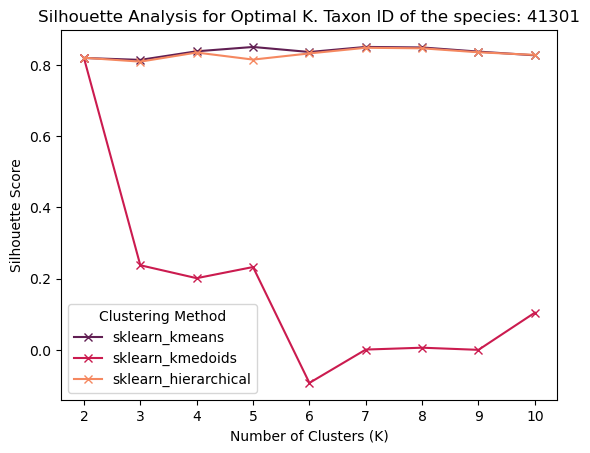
\includegraphics[width=\textwidth]{figures/sil_score.png}
        \caption{Silhouette scores for different clustering algorithms applied to data from a species (Taxon ID: 41301). This analysis was performed on all species present in Florida from the dataset.}
        \label{fig:sil_score}
    \end{minipage}\hfill
    \begin{minipage}{0.49\textwidth}
        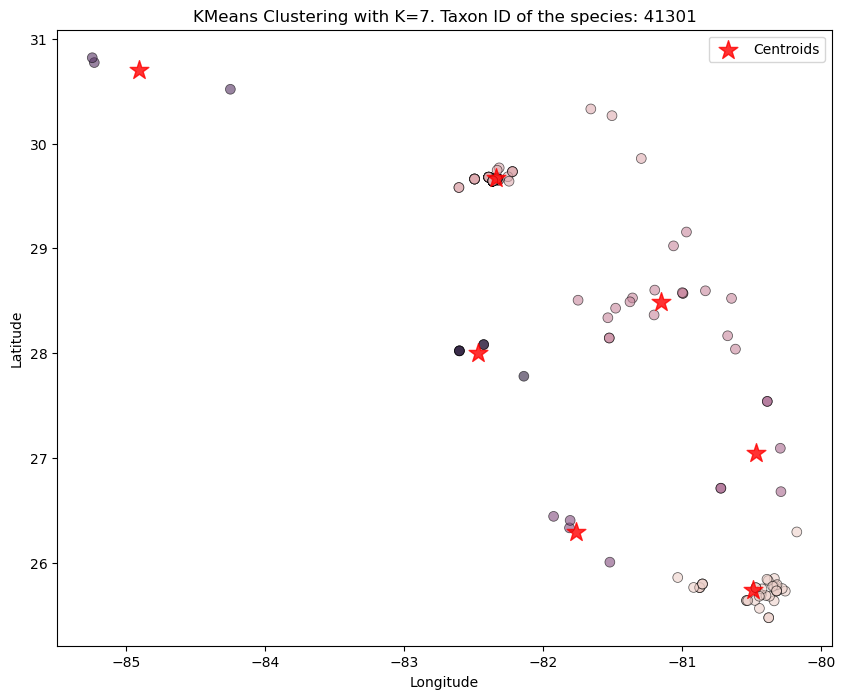
\includegraphics[width=\textwidth]{figures/cluster_map.png}
        \caption{Map illustrating subpopulations in Florida (Taxon ID: 1997) clustered with k-means algorithm. Silhouette Score: 0.85 for 7 clusters.}
        \label{fig:cluster_map}
    \end{minipage}\hfill
\end{figure}
\begin{table}[h!]
\centering
\begin{minipage}{\textwidth}
\begin{tabular}{lcc}
\toprule
\textbf{Method} & \textbf{Silhouette Score} & \textbf{Optimal Number of Clusters} \\
\midrule
\texttt{sklearn\_kmeans}       & 0.850965 & 7 \\ 
\texttt{sklearn\_kmedoids}     & 0.819892 & 2 \\ 
\texttt{sklearn\_hierarchical} & 0.848580 & 7 \\ 
\bottomrule
\end{tabular}
\caption{Maximum Silhouette Scores (from Figure \ref{fig:sil_score}) indicating the optimal number of clusters for different clustering algorithms applied to the dataset of a species (Taxon ID: 41301).}
\label{tab:clustering_results}
\end{minipage}
\end{table}


\subsection{Decision Tree Classification}
The Adaboosted Decision tree model showed the best performance in both accuracy and F1-score, and testing a number of estimators from 50-200 and learning rate from 0.01 to 10 showed no increase in performance from the base model (Table \ref{tab:ensemble_results}). When training on more imbalanced data such as species \textit{Oceanites oceanicus} (species ID: 4146) with 0.94\% presence, the AdaBoosted decision tree performs poorer (F1: 0.12) than the base estimator tree (F1: 0.2) as it predicts more positive instances. Despite this, this model correctly identifies the coastal distribution of the target species, with some predictions biased by a single outlier that is seen in the training data. (Figures \ref{fig:pred1}-\ref{fig:pred3}) This is preferred over producing too few positive labels as it shows the model is not over-fit and is able to output new environmentally suitable locations. For widely distributed species such as \textit{Tyrannus tyrannus} (species ID: 16782), the AdaBoosted decision tree performs equally to the base decision tree (F1: 0.86). Both models correctly identify absence on the west coast, with the AdaBoosted tree more biased toward predicting absences. Both models are biased by the pseudo-absences in southern Florida that are seen in the training data.

\begin{figure}[H]
    \begin{minipage}{0.3\textwidth}
        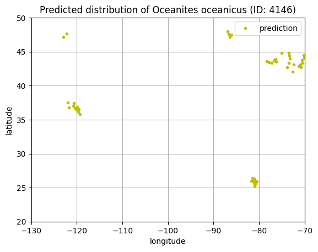
\includegraphics[width=\textwidth]{figures/decision_tree.png}
        \caption{Base Decision Tree prediction of Species ID 4146 presence.}
        \label{fig:pred1}
    \end{minipage}\hfill
    \begin{minipage}{0.3\textwidth}
        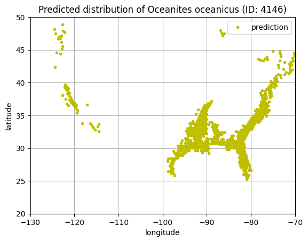
\includegraphics[width=\textwidth]{figures/adaboost.png}
        \caption{AdaBoost prediction of Species ID 4146 presence.}
        \label{fig:pred2}
    \end{minipage}\hfill
    \begin{minipage}{0.3\textwidth}
        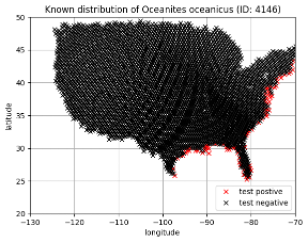
\includegraphics[width=\textwidth]{figures/test_species.png}
        \caption{Test data distribution of Species ID 4146 presence.}
        \label{fig:pred3}
    \end{minipage}\hfill
\end{figure}

\subsection{Co-occurence Clustering}
In an example analysis of the species \textit{Oceanites oceanicus} (species ID: 4146), we observe its highest occurence in a single cluster out of the nine outputted by K-Means (Figure \ref{fig:kmeansclust}). Using a list of the five most abundant species in said cluster, Taxon IDs: [26159, 19765, 12024, 41301, 4765], we output a KDE plot that is able to qualitatively rank potential areas of relocation. In this case, there is a seemingly tight relationship between the areas of species clustering, and the areas of habitat based prediction.

\begin{figure}[H]
    \begin{minipage}{0.49\textwidth}
        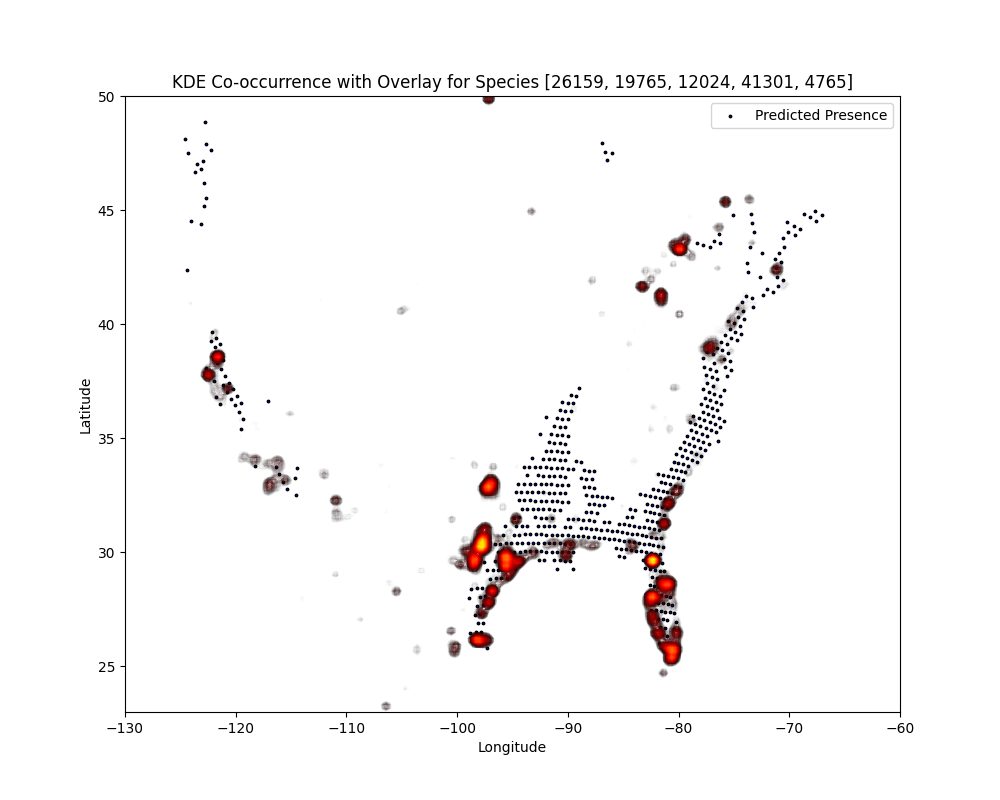
\includegraphics[width=\textwidth]{figures/4146_Overlay.png}
        \caption{Overlaid KDE Plot of Species ID 4146. Yellow areas represent higher co-occurence.}
        \label{fig:overlay1}
    \end{minipage}\hfill
    \begin{minipage}{0.49\textwidth}
        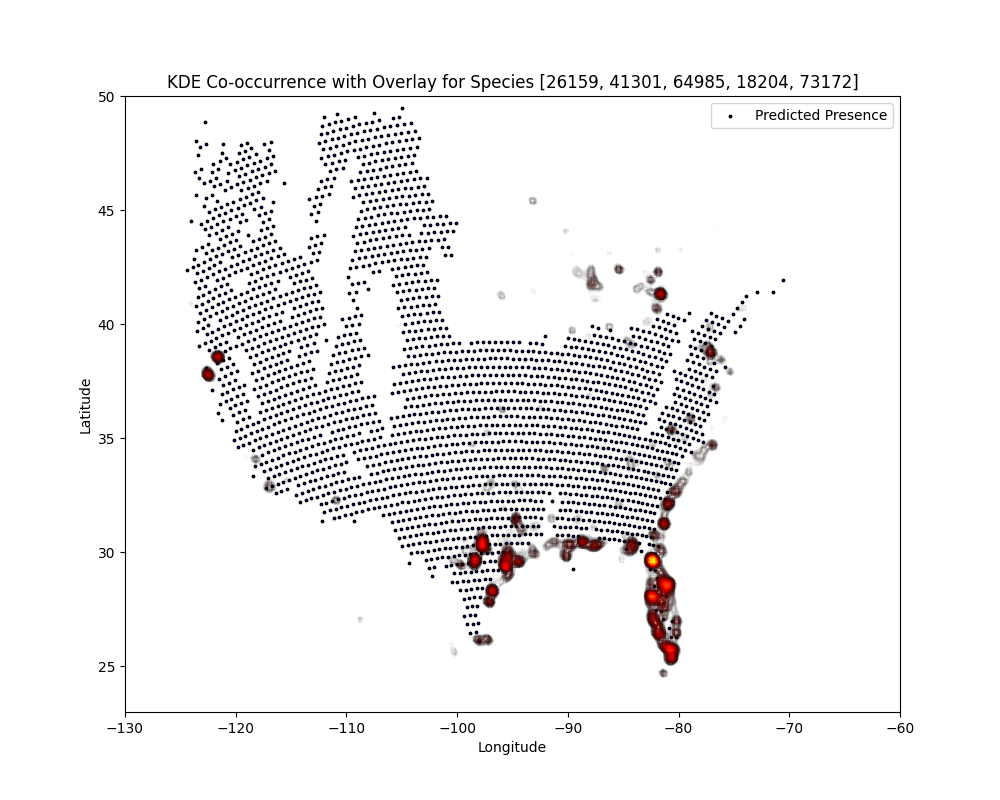
\includegraphics[width=\textwidth]{figures/41301_Overlay.png}
        \caption{Overlaid KDE Plot of Species ID 41301. Yellow areas represent higher co-occurrence.}
        \label{fig:overlay2}
    \end{minipage}\hfill
\end{figure}

However, analysing the species \textit{Tadarida brasiliensis} (species ID: 41301) while adjusting for reallocation to similar fauna outputs a significantly reduced set of possible translocations from the list of predictions. 

\section{Conclusions}
\textbf{Subpopulation clustering:} Clustering provides insights into the possible distribution of species subpopulations in Florida that may be useful in identifying groups impacted by natural hazards. Silhouette Score was used to evaluate and compare clusters produced with different clustering algorithms.

\textbf{Decision Tree Classification:}
AdaBoosted decision trees identify locations that are environmentally suitable for target species with only a few observations. It suffers from bias towards few outliers in the training data, but too many false positives is preferred over too few.

\textbf{Fauna Based Prediction:} The clustering outputs used in making the Kernel Density Estimation plot are able to qualitatively provide a usable subset of regions of similar biodiversity. In addition to the habitat based predictive model, it is able to act as a layer of ranking and validation for output from Decision Tree classification with few false positives. For species with a very high proportion of false positives, the KDE is able to collapse the output of the Habitat Based Predictor to a usable set. 

A potential critique of this model is that it works under two main assumptions: 

1) The habitat and climate of the target location is suitable for long term translocation and conservation attempts

2) Conservation attempts largely aim to have slightly different biomes that can allow a target species to grow and reproduce (e.g., lesser natural predator species), however, this model does not capture that due to a lack of availability of species interactomes\cite{MORRIS2021e01630}.

\newpage
\section*{Individual contribution statement}
\begin{itemize}
    \item s2013679: Contributed to data preparation (organising original data, fetching climate and elevation data for concatenation, use of a K-nearest neighbours classifier.)
    \item s2713107: Contributed to researching different clustering algorithms (k-means, k-medoids, hierarchal), computing silhouette scores and visualising clusters on a map.
    \item s2691680: Contributed to researching and writing background in introduction and abstract, and developing the decision tree classifiers.
    \item s2762009: Clustering across all species, kernel density estimation graphs, researching and writing background and conclusion
\end{itemize}    
\section*{Use of AI declaration}
ChatGPT was occasionally used to help identify sources of error in our Python code.

\newpage
\bibliography{refs.bib}
\bibliographystyle{plain}

\newpage
\section*{Appendix} \label{appendix}
\renewcommand{\thefigure}{A\arabic{figure}}
\setcounter{figure}{0}

\subsection*{Data and code}
Original resources relevant to the project report can be found in the Supplementary Material archive ("21.zip").

\subsection*{Additional material}
\begin{figure}[H]
    \centering
    \begin{minipage}{0.90\textwidth}
        \centering
        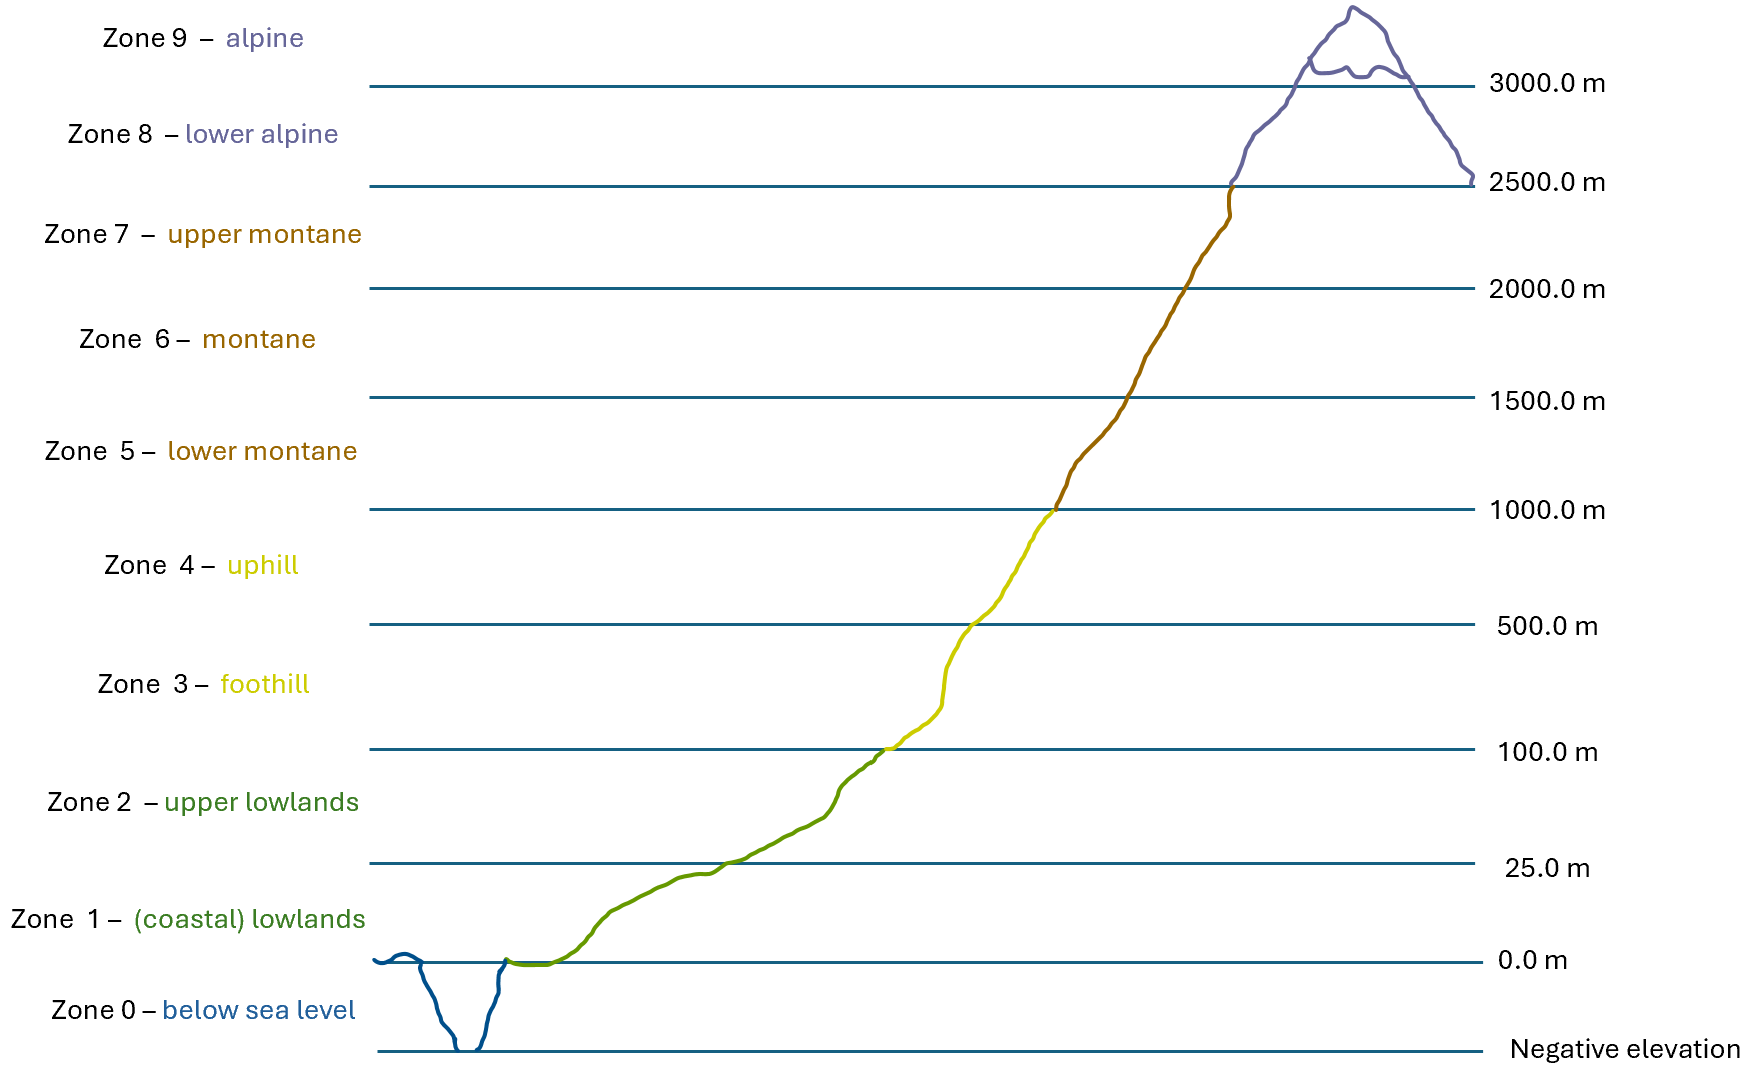
\includegraphics[width=\textwidth]{figures/elevationzonation.png}
        \caption{Schematic of the ordinal elevation zones defined in the data.}
        \label{fig:elevations}
    \end{minipage}\hfill
\end{figure}

\begin{figure}[H]
\begin{minipage}{0.90\textwidth}
        \centering
        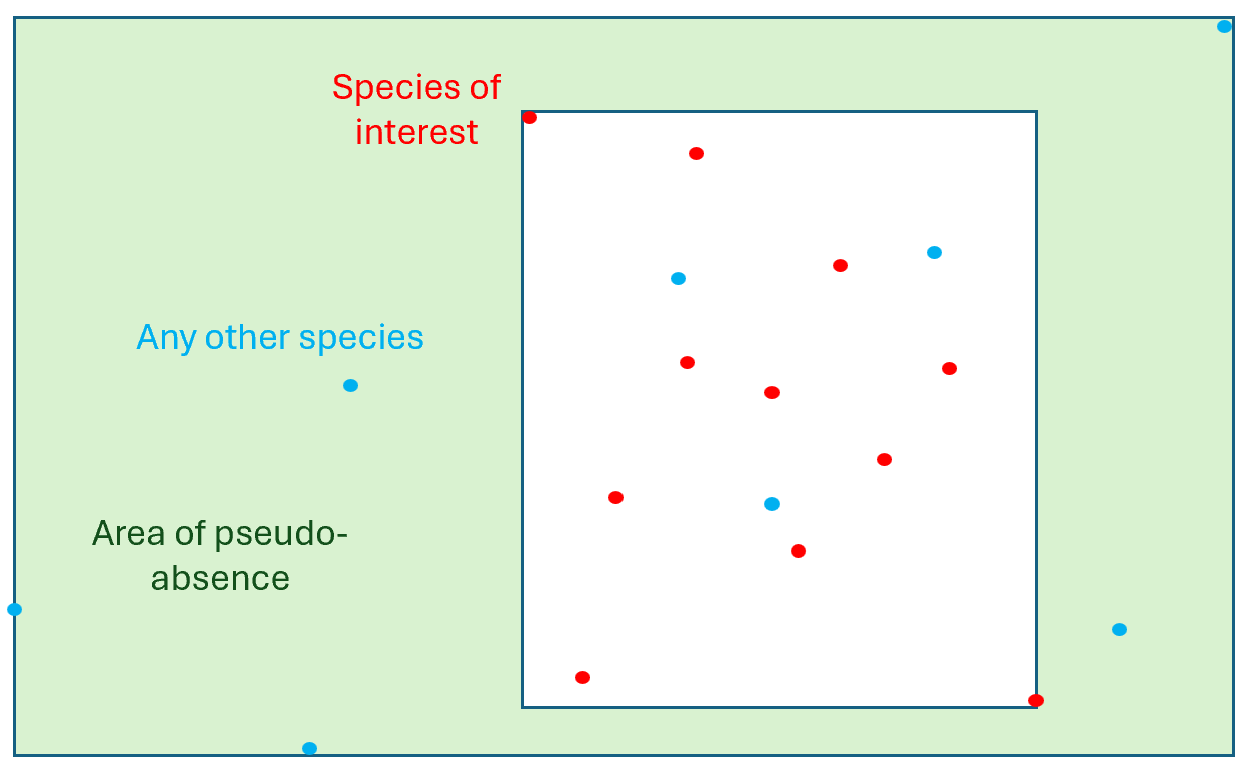
\includegraphics[width=\textwidth]{figures/boxdifference.png}
        \caption{Diagram of the box-difference pseudo-absence sampling method.}
        \label{fig:absences}
    \end{minipage}
\end{figure}

\begin{figure}[H]
    \centering
    \begin{minipage}{0.9\textwidth}
        \centering
        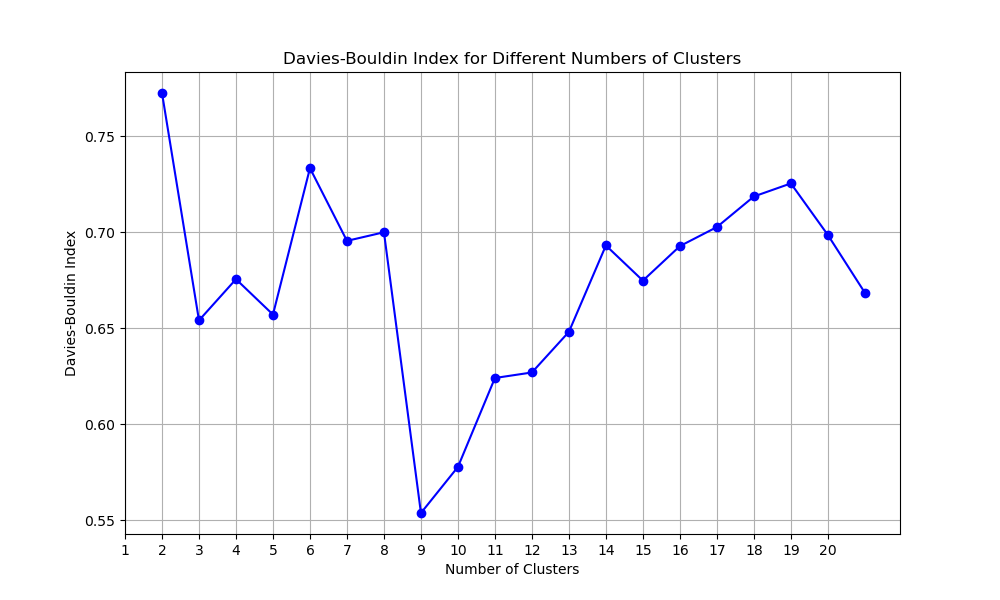
\includegraphics[width=\textwidth]{figures/kmeandbi.png}
        \caption{Davies-Bouldin Indices for K-Means Clustering for all species in Florida}
        \label{fig:kmeansdbi}
    \end{minipage}
\end{figure}

\begin{figure}[H]
    \centering
    \begin{minipage}{0.9\textwidth}
        \centering
        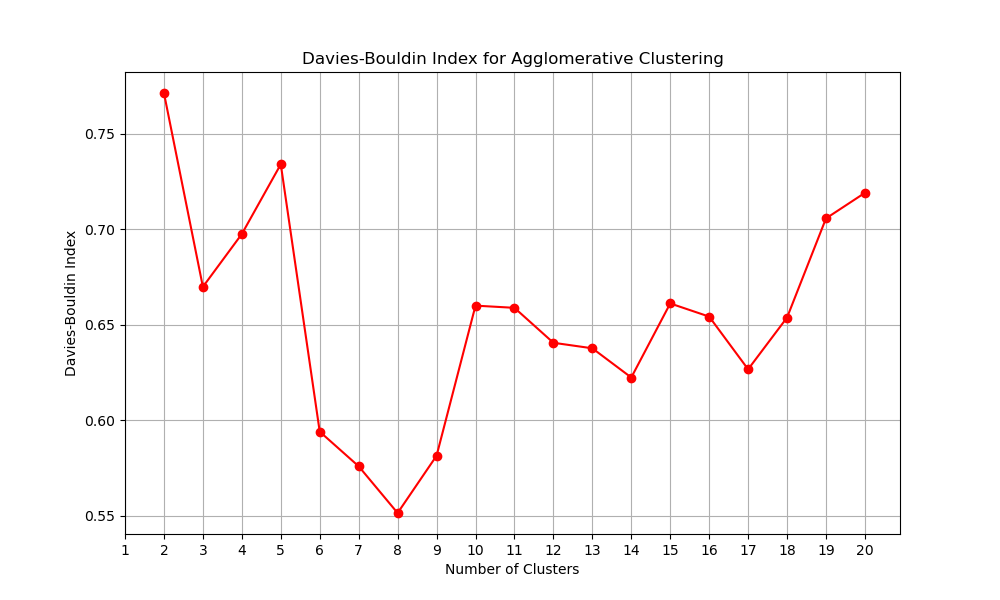
\includegraphics[width=\textwidth]{figures/aggdbi.png}
        \caption{Davies-Bouldin Indices for Agglomerative Clustering for all species in Florida}
        \label{fig:aggdbi}
    \end{minipage}
\end{figure}


\begin{figure}[H]
    \centering
    \begin{minipage}{0.9\textwidth}
        \centering
        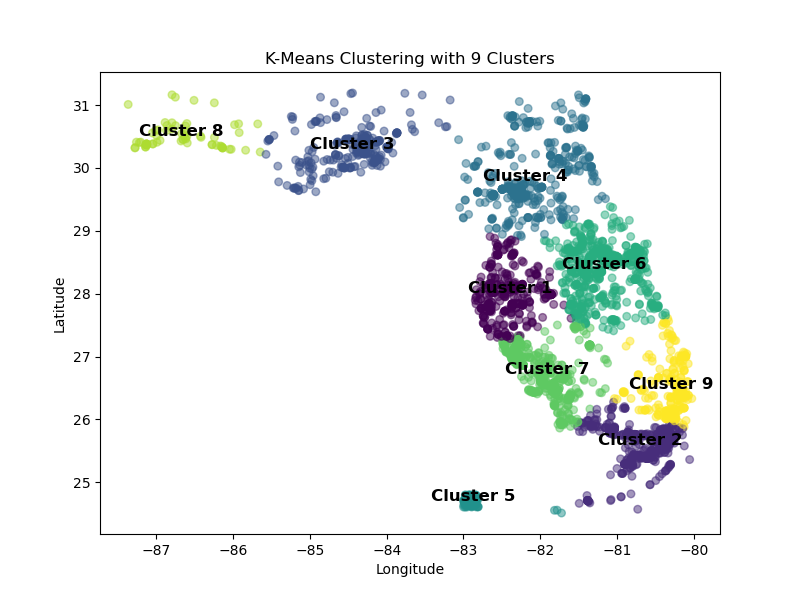
\includegraphics[width=\textwidth]{figures/ninecluster.png}
        \caption{K-Means Clustering with 9 Clusters for all species in Florida}
        \label{fig:kmeansclust}
    \end{minipage}
\end{figure}


\end{document}

%%% Local Variables:
%%% mode: latex
%%% TeX-master: t
%%% End:
